\documentclass{article}
\usepackage{fancyhdr}
\usepackage{lipsum}  
\usepackage{listings} 
\usepackage{xcolor}   
\usepackage{amsmath}
\usepackage{enumitem}

% Define macros for title and author
\newcommand{\thetitle}{MATH 417 502 HW6}
\newcommand{\theauthor}{Keegan Smith}

\title{\thetitle}
\author{\theauthor}

\pagestyle{fancy}
\fancyhf{}  % Clear all header and footer fields
\fancyhead[L]{\nouppercase{\rightmark}}
\fancyhead[C]{\thetitle}  % Title in the center
\fancyhead[R]{\theauthor}  % Your name on the right
\usepackage{amsmath}
\usepackage{graphicx}
\usepackage[colorlinks=true, allcolors=blue]{hyperref}
\lstset{ %
  backgroundcolor=\color{white},   % choose the background color
  basicstyle=\ttfamily\small,          % size of fonts used for the code
  keywordstyle=\color{black},           % color for keywords
  commentstyle=\color{black},          % color for comments
  stringstyle=\color{black},             % color for strings
  numbers=left,                        % where to put the line-numbers
  numberstyle=\tiny\color{gray},       % style for line-numbers
  stepnumber=1,                        % the step between two line-numbers
  numbersep=5pt,                       % how far the line-numbers are from the code
  frame=single,                        % adds a frame around the code
  rulecolor=\color{black},             % frame color
  breaklines=true,                     % automatic line breaking
  breakatwhitespace=false,             % automatic breaks should only happen at whitespace
  showspaces=false,                    % don't show spaces in the code
  showstringspaces=false,              % don't show spaces in strings
  showtabs=false,                      % don't show tabs in the code
}
\begin{document}
\maketitle
\section* {Problem 1}
for h=.0004:
\begin{figure}[!h]
\centering
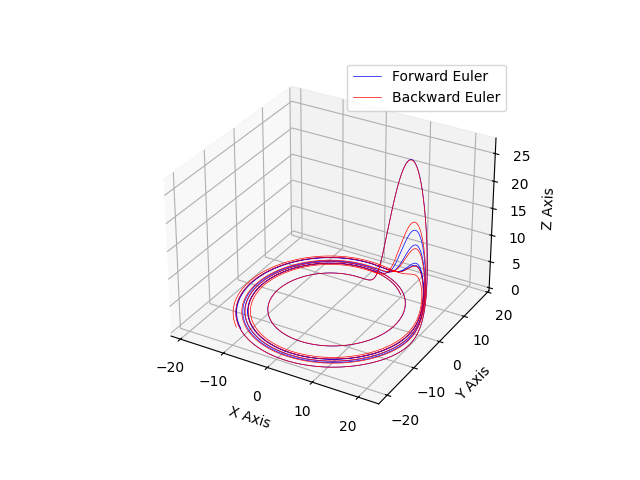
\includegraphics[width=1.0\textwidth]{figs/both.png}
\end{figure}
\newpage
I found that a very small step size h=.00004 causes backward and forward euler to be nearly equivalent. When h is large, forward euler blows up. Backward euler does not seem to blow up as quickly. 
\begin{lstlisting}
import numpy as np
import matplotlib.pyplot as plt
from mpl_toolkits.mplot3d import Axes3D

def plot_rossler_attractor(results, title):
    x = [result[0] for result in results]
    y = [result[1] for result in results]
    z = [result[2] for result in results]

    fig = plt.figure()
    ax = fig.add_subplot(111, projection='3d')
    ax.plot(x, y, z, lw=0.5)

    ax.set_xlabel("X Axis")
    ax.set_ylabel("Y Axis")
    ax.set_zlabel("Z Axis")
    ax.set_title(title)
    plt.savefig("figs/" + title + ".png")
def plot_rossler_both(backward_results, forward_results):
    x_f = [result[0] for result in forward_results]
    y_f = [result[1] for result in forward_results]
    z_f = [result[2] for result in forward_results]

    x_b = [result[0] for result in backward_results]
    y_b = [result[1] for result in backward_results]
    z_b = [result[2] for result in backward_results]

    fig = plt.figure()
    ax = fig.add_subplot(111, projection='3d')

    ax.plot(x_f, y_f, z_f, lw=0.5, color='blue', label='Forward Euler')

    ax.plot(x_b, y_b, z_b, lw=0.5, color='red', label='Backward Euler')

    ax.set_xlabel("X Axis")
    ax.set_ylabel("Y Axis")
    ax.set_zlabel("Z Axis")

    ax.legend()
    plt.savefig("figs/both.png")
    #plt.show()
def function_a(y_n):
    a = .1
    b = .1
    c = 14
    if(len(y_n) != 3):
        raise RuntimeError("input vector for function a does not equal 3")
    result = [0.0] * 3;
    result[0] = -y_n[1] - y_n[2];
    result[1] = y_n[0] + a * y_n[1]
    result[2] = b + y_n[2] * (y_n[0] - c);
    return result;
def jacobian_a(y_n):
    a = .1
    b = .1
    c = 14
    if(len(y_n) != 3):
        raise RuntimeError("input vector for jacobian a does not equal 3")
    result = [
        [-1, -1, 0],
        [1, a, 0],
        [y_n[2], 0, y_n[0] - c]
    ]
    return result;
def G(y_n:list, h: float, f, z: list):
    function_result = f(z);
    if(len(function_result) != len(z) or len(function_result) != len(y_n)):
        raise RuntimeError("vector sizes do not match in function G")
    result = [0.0] * len(y_n)
    for i in range(0, len(y_n)):
        result[i] = y_n[i] + h * function_result[i] - z[i]
    return result;
def G_jacobian(y_n: list, h: float, f_prime, z: list):
    function_result = f_prime(z);
    for i in range(0, len(function_result)):
        for j in range(0, len(function_result[i])):
            function_result[i][j] *= h;
            if(i == j):
                function_result[i][j] -= 1
    return function_result;
    
def forward_euler_iteration(y_n : list, h: float, f):
    function_result = f(y_n)
    if(len(function_result) != len(y_n)):
        raise RuntimeError("vector sizes do not match in forward euler.")
    result = [0.0] * len(y_n);
    for i in range(0, len(y_n)):
        result[i] = y_n[i] + h * function_result[i]
    return result;
def run_forward_euler(y_n : list, h: float, f, num_iterations: int):
    results = [y_n]
    for i in range(0, num_iterations):
        y_n = forward_euler_iteration(y_n, h, f)
        results.append(y_n);
    return results;
def backward_euler_iteration(y_n: list, h: float, f, f_prime, z: list):
    jacobian = G_jacobian(y_n, h, f_prime, z)
    g_vector = G(y_n, h, f, z)
    product = np.linalg.solve(jacobian, g_vector)
    next_z = [0.0] * len(product)
    for i in range(0, len(product)):
        next_z[i] = z[i] - product[i]
    result = [0.0] * len(product)
    function_result = f(next_z)
    for i in range(0, len(product)):
        result[i] = y_n[i] + h * function_result[i]
    return result, next_z

def run_backward_euler(y_n: list, h: float, f, f_prime, num_iterations: int):
    z = y_n;
    results = []
    for i in range(0, num_iterations):
        y_n, z = backward_euler_iteration(y_n, h, f, f_prime, z)
        results.append(y_n)
    return results

def main():
    num_iterations = 100000;
    y_0 = [10.0, 10.0, 0.0]
    time_interval = [0, 40]
    h = (time_interval[1] - time_interval[0]) /num_iterations
    print("h is: ", h)
    print("Performing forward euler:")
    forward_euler_results = run_forward_euler(y_0, h, function_a, num_iterations)
    #print(forward_euler_results)
    plot_rossler_attractor(forward_euler_results, "forward euler")
    
    print("Performing backward euler:")
    y_0 = [10.0, 10.0, 0.0]
    backward_euler_results = run_backward_euler(y_0, h, function_a, jacobian_a, num_iterations)
    #print(backward_euler_results)
    plot_rossler_attractor(backward_euler_results, "backward euler")
    plot_rossler_both(backward_euler_results, forward_euler_results)
if __name__ == "__main__":
    main();
\end{lstlisting}
\section*{Problem 2}
\begin{enumerate}
\item We want a system of equations such that $\frac{d}{dt}y_n(t) = y_{n+1}(t)$. Thus we will have: \\
\begin{align*}
y_1(t) &= y(t) \\
y_2(t) &= y'(t) \\
y_3(t) &= y''(t) \\
y_4(t) &= y'''(t)
\end{align*}
Plugging in the values from the given equation: \\
\begin{align*}
y_4'(t) &= t^2 - 3 \cdot y_3(t) + \sin (t) \cdot y_2(t) - 8 \cdot y_1(t) \\
y_3'(t)  &= y_4(t) \\
y_2'(t) &= y_3(t) \\
y_1'(t) &= y_2(t)\\
\end{align*}
Thus we have $y'(t) = f(t, x)$ where: \\
\[
f(t,x) =
\begin{cases}
x_2(t) \\
x_3(t) \\
x_4(t) \\
t^2 - 3 \cdot x_3(t) + \sin (t) \cdot x_2(t) - 8 \cdot x_1(t) \\
\end{cases} 
\]
\item For backward euler we have: \\
\begin{align*}
y_{n+1} &= y_n + h \cdot f(t_{n+1}, y_{n+1})\\
\end{align*}
where $f$ is the same function as we derived above. \\
To find the $y_{n+1}$ on the rightside we will use newton iteration: \\
\begin{align*}
0 &= y_n + h \cdot f(t_{n+1}, y_{n+1}) - y_{n+1} \\
0 &= y_n + h \cdot f(t_{n+1}, z) - z \quad \mbox{Substituting $y_{n+1}$ with $z$}
\end{align*}
Thus we are finding the root of the function: \\
\begin{align*}
G(z) &=  y_n + h \cdot f(t_{n+1}, z) - z \\
G(z) &= \begin{bmatrix}
y_1 + h \cdot z_2(t) - z_1(t) \\
y_2 + h \cdot z_3(t) - z_2(t) \\
y_3 + h \cdot z_4(t) - z_3(t) \\
y_4 + h \cdot t^2 - 3 \cdot z_3(t) + \sin (t) \cdot z_2(t) - 8 \cdot z_1(t) - z_4(t) \\
\end{bmatrix}
\end{align*}
Recall the newton scheme is given by: \\
\[
y_{n+1} = y_n - (J^{-1}F(z))F(z)
\]
The jacobian of $G(z)$ is:\\
\[
JG(z) = \begin{bmatrix}
-1 & h & 0 & 0 \\
0 & -1 & h & 0 \\
0 & 0 & -1 & h \\
-8 & sin(t) & -3 & -1 \\
\end{bmatrix}
\]
Thus we have: \\
\[
z_{n+1} = y_n - \begin{bmatrix}
-1 & h & 0 & 0 \\
0 & -1 & h & 0 \\
0 & 0 & -1 & h \\
-8 & sin(t) & -3 & -1 \\
\end{bmatrix}^{-1}
\begin{bmatrix}
y_1 + h \cdot z_2(t) - z_1(t) \\
y_2 + h \cdot z_3(t) - z_2(t) \\
y_3 + h \cdot z_4(t) - z_3(t) \\
y_4 + h \cdot t^2 - 3 \cdot z_3(t) + \sin (t) \cdot z_2(t) - 8 \cdot z_1(t) - z_4(t) \\
\end{bmatrix}
\]
And whatever we get for $z_{n+1}$ we plug into $y_{n+1}$ on the rightside of the original backward euler scheme. We can then evaluate that equation to find the true $y_{n+1}$.
\end{enumerate}
\end{document}